% !TeX spellcheck = hu_HU
%----------------------------------------------------------------------------
\chapter{Wireframe-ek}
%----------------------------------------------------------------------------

A wireframe–ek egy alkalmazás tervezésénél nagyon gyakran elmaradnak, pedig igenis fontos szerepük van.
Rengeteg olyan dologra világíthatnak rá, amire egyébként nem gondolnánk és segíti a kommunikációt a fejlesztő(k) és a megrendelő között.

A dolgozatba csak a főbb képernyők wireframe–ét helyeztem el. Ezeknek az elkészítéséhez a Figma \footnote{A Figma hivatalos weboldala: \url{https://figma.com/}}. névre keresztelt webes alkalmazást használtam. 
Ennek segítségével az egyszerű wireframe–ektől kezdve komplex prototipizált design terveket is készíthetünk.

\section{Bejelentkezés és regisztráció}
A bejelentkezés és regisztráció oldalak (\refstruc{fig:RegistrationWireframe}) felépítése azonos, egyedül a beviteli mezőkben térnek el.
A navigációs sávban csak a bejelentkezés és a regisztráció opciók közül választhatunk. A képernyő közepén mind a két esetben egy formot jelenítünk meg a szükséges adatokat bekérő beviteli mezőkkel.
\begin{figure}[!ht]
  \centering
  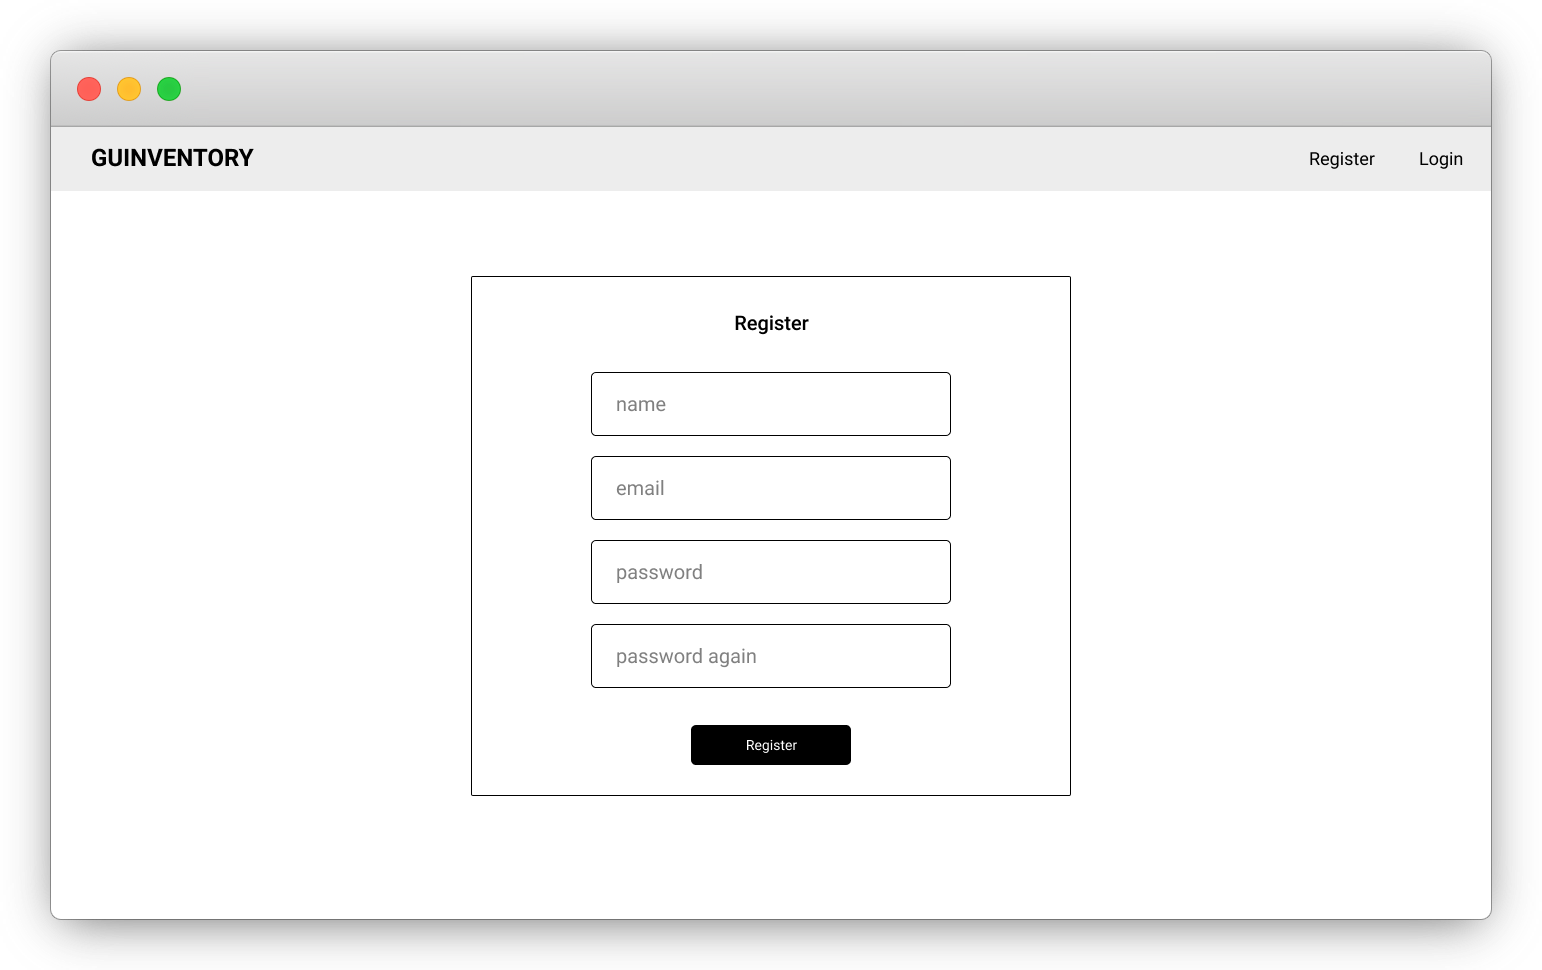
\includegraphics[width=150mm, keepaspectratio]{figures/wireframes/frame_registration.png}
  \caption{Regisztráció wireframe}
  \label{fig:RegistrationWireframe}
\end{figure}


\section{Keresés}
A keresést, annak érdekében, hogy az alkalmazás bármely részéről könnyedén elérhető legyen a felső navigációs sávba helyeztem el.
A wireframe (\refstruc{fig:SearchWireframe}) alapján látszik, hogy kereséskor egy legördülő listában jelennek meg az eredmények, így az aktuális oldal elhagyása nélkül láthatjuk a keresett eszköz helyét.
\begin{figure}[!ht]
  \centering
  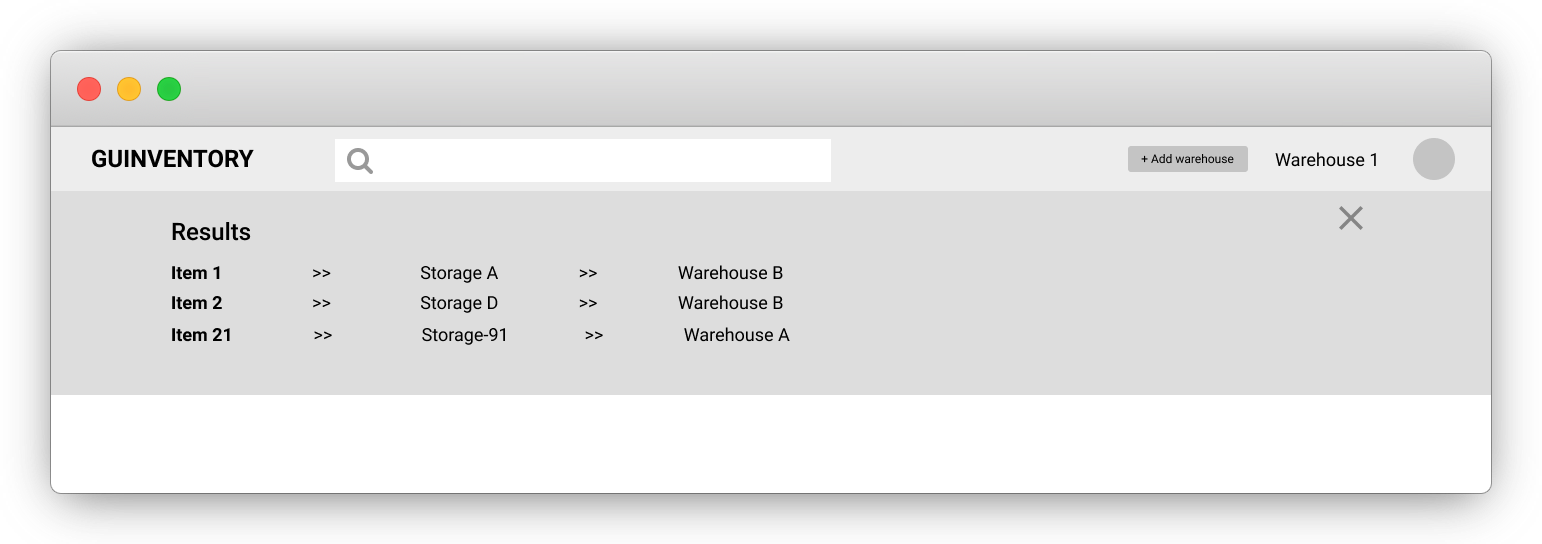
\includegraphics[width=150mm, keepaspectratio]{figures/wireframes/search.png}
  \caption{Keresés wireframe}
  \label{fig:SearchWireframe}
\end{figure}


\section{Raktár nézet}
A raktár oldalán (\refstruc{fig:WarehouseWireframe}) láthatunk egy térképes nézetet és egy listát is a tárolókról. 
A térképes nézeten a kurzort a tároló fülé mozgatva megjelenítjük annak nevét a könnyebb azonosítás érdekében.

Ezen felül a navigációs sávban láthatjuk az éppen kiválasztott raktárat, ahol egy legördülő menü segítségével azonnal választhatunk másik raktárat is, amennyiben több raktárhoz is van hozzáférésünk.
A raktár választó mellett megjelenítünk egy gombot, amellyel új tárolót hozhatunk létre.
\begin{figure}[!ht]
  \centering
  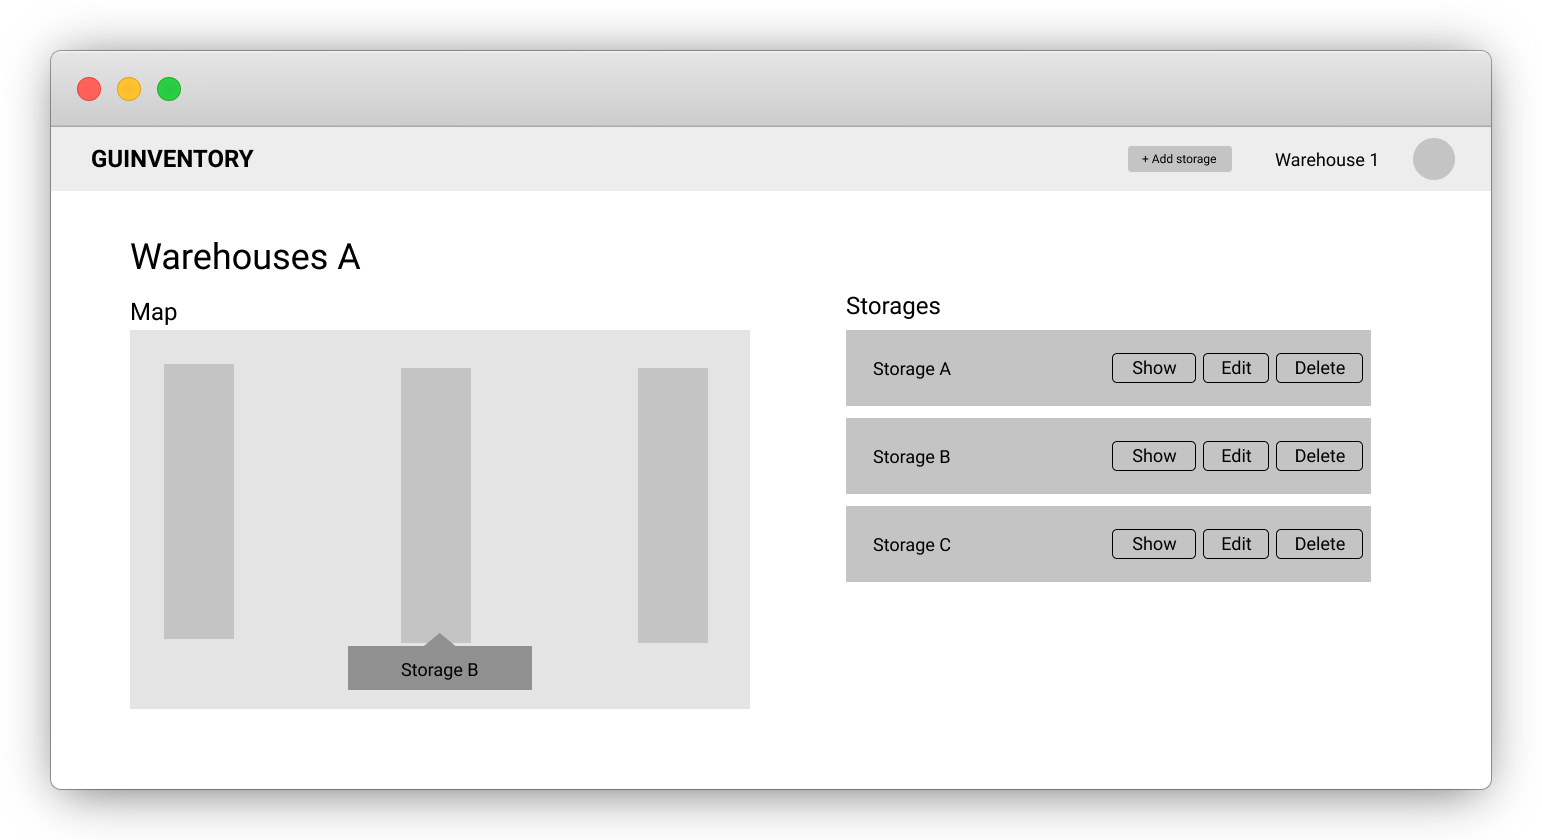
\includegraphics[width=150mm, keepaspectratio]{figures/wireframes/frame_warehouse.png}
  \caption{Raktár wireframe}
  \label{fig:WarehouseWireframe}
\end{figure}

\section{Tároló nézet}
A tároló nézete (\refstruc{fig:StorageWireframe}) nagyon hasonlít a raktáréhoz, azonban itt kiegészítésként a térkép felett megjelenítünk egy másik tárolót is.
Ez a feladatspecifikációban megkövetelt tárolók közötti eszköz mozgatását teszi lehetővé.

A navigációs sávban itt is megjelenítjük a raktár választó gombot, azonban a tároló létrehozása helyett, itt az eszköz felvétele gombot találhatjuk.

\begin{figure}[!ht]
  \centering
  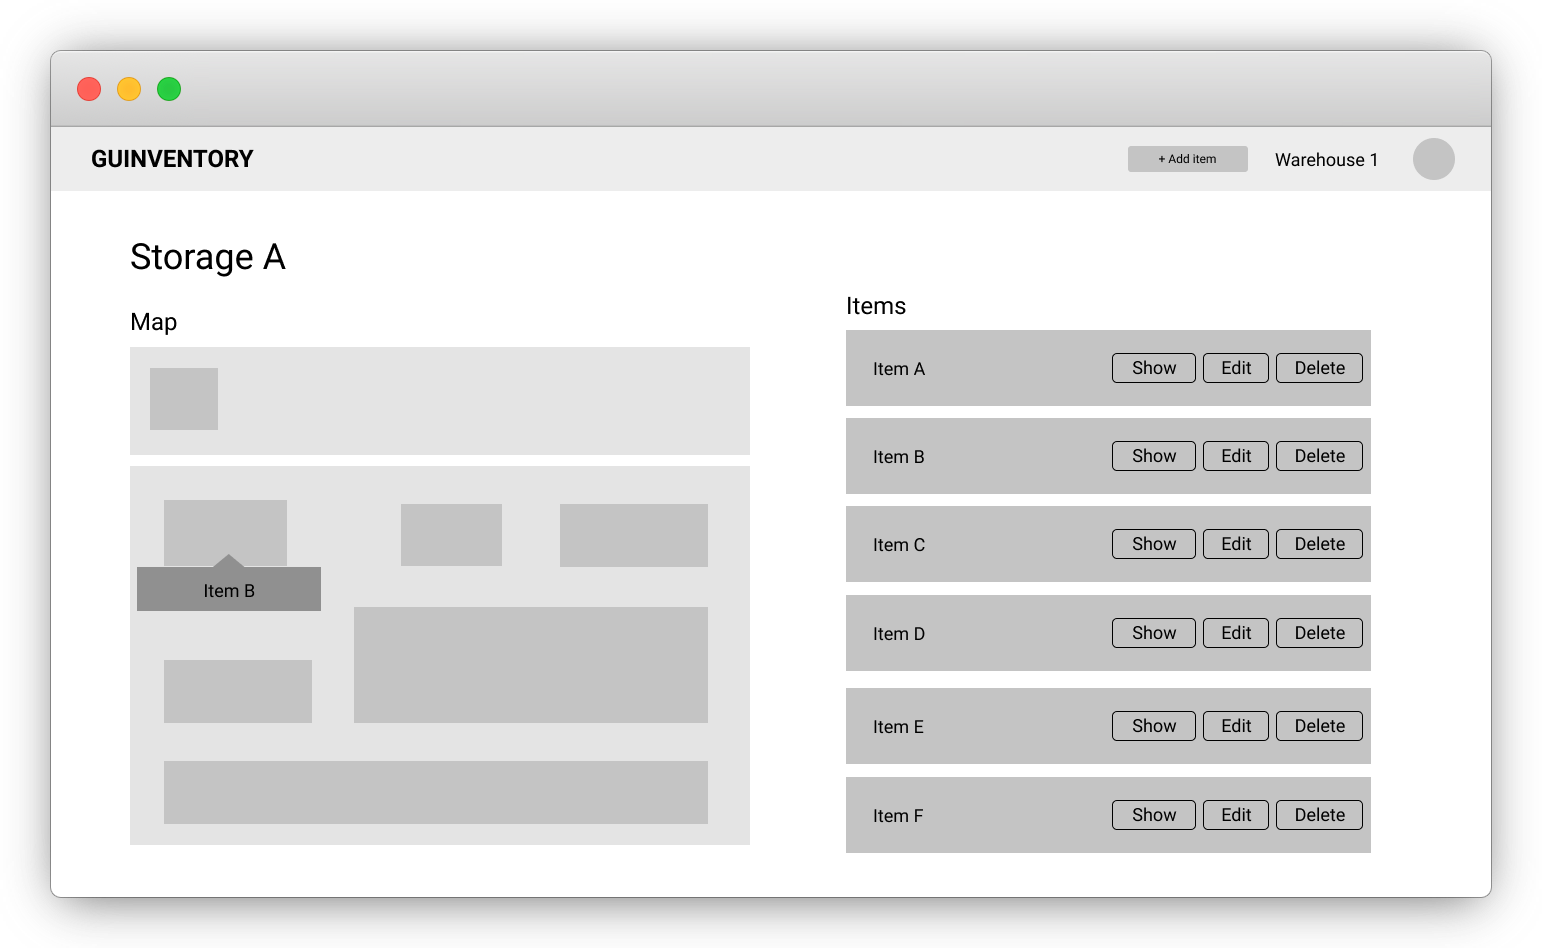
\includegraphics[width=150mm, keepaspectratio]{figures/wireframes/frame_storage.png}
  \caption{Tároló wireframe}
  \label{fig:StorageWireframe}
\end{figure}
  